\normalfalse \difficiletrue \tdifficilefalse
\correctiontrue

%\UPSTIidClasse{11} % 11 sup, 12 spé
%\newcommand{\UPSTIidClasse}{11}

\exer{Pèse camion  $\star\star$ \label{C1:05:57}}
\setcounter{question}{0}\UPSTIcompetence[2]{C1-05}
\index{Compétence C1-05}
\index{PFS}
\index{Pèse camion}
\ifcorrection
\else
\marginnote{\textbf{Pas de corrigé pour cet exercice.}}
\fi

\ifprof
\else
On considère un bâti \textbf{0} auquel est attaché le repère$\mathcal{R}=\left(O;\vect{x_0};\vect{y_0};\vect{z_0} \right)$. Le champ de pesanteur est $g=-g\vect{y_0}$.La barre \textbf{1} est liée au bâti \textbf{0} par une liaison pivot parfaite d’axe $\left(A,\vect{z_0}\right)$. Le plateau porte camion \textbf{2} est lié à la barre \textbf{1} par une liaison pivot parfaite d’axe $\left(C,\vect{z_0}\right)$. Le levier \textbf{3} est lié au bâti \textbf{0} par une liaison pivot parfaite d’axe $\left(B,\vect{z_0}\right)$. Ce levier est également lié au plateau \textbf{2} par une liaison pivot parfaite d’axe $\left(D,\vect{z_0}\right)$. Le camion \textbf{4}, de centre de masse $G$ et de masse $M$ inconnue, repose sur le plateau \textbf{2}.
L’action mécanique connue est caractérisée par : $\{\text{ext}\rightarrow 3\}=\left\{
\begin{array}{c}
-F\vect{y_0} \\
\vect{0} \\
\end{array}
\right\}_E$ .


\begin{center}
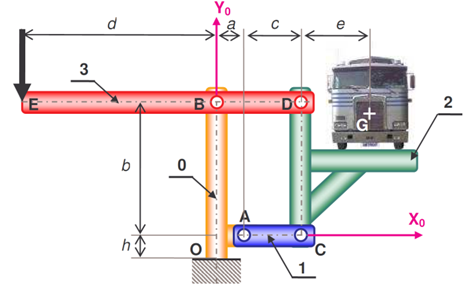
\includegraphics[width=\linewidth]{57_01}
\end{center}


\fi

\question{Tracer le graphe de structure. Définir le nombre d'inconnues statiques.}
\ifprof

\begin{center}
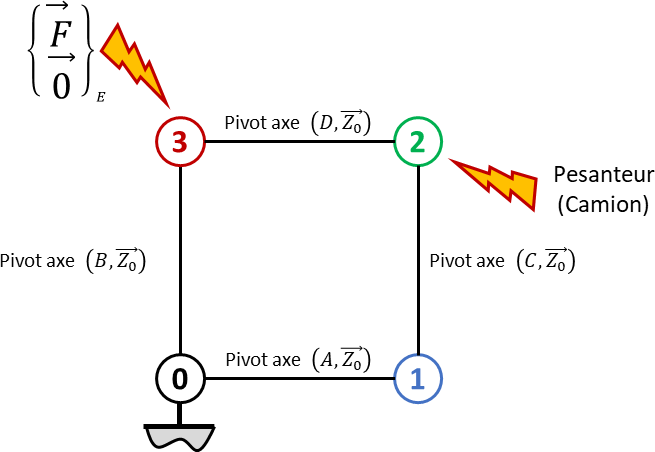
\includegraphics[width=10cm]{57_01_Cor}
\end{center}

En faisant l'hypothèse de problème plan, on a 8 inconnues statiques. 
\else
\fi



\question{Donner la stratégie permettant de déterminer la valeur de $F$ en fonction de $M$.}
\ifprof
\begin{itemize}
\item On commence par isoler \textbf{1} soumis à 2 glisseurs. D'après le PFS, les actions mécaniques en $A$ et en $C$ sont dirigées suivant la direction $\vect{x_0}$.
\item On isole ensuite \textbf{2}. Le solide \textbf{2} étant en translation circulaire, on réalise un TRS suivant $\vect{y_0}$. 
\item On isole enfint \textbf{3}. Le solide \textbf{3} étant en rotation autour de $\axe{B}{z_0}$ par rapport à \textbf{0},  on réalise un TMS en $B$ suivant $\vect{z_0}$. 
\end{itemize}
\else
\fi
\ifprof
\else
\begin{flushright}
\footnotesize{Corrigé  voir \ref{C1:05:57}.}
\end{flushright}%
\fi